\section{معماری پیشنهادی}
در ابتدا همان طور که گفته شد در این معماری سعی می‌کنیم که تا جای ممکن از معماری
\lr{event driven}
استفاده کنیم. به عنوان مثال برای شروع اولین کاری که می‌توان کرد این است که به جای اینکه با کاوه‌نگار و پاکت
و زرینپال به صورت مستقیم در ارتباط باشیم از یک صف استفاده کنیم. در همه‌ی
\lr{usage}های
کاوه‌نگار و پاکت استفاده از صف منطقی است ولی زرینپال کمی داستانش فرق می‌کند و بعضی جا‌ها نمی‌توان از
صف استفاده کرد که در ادامه‌ی این قسمت به آن می‌پردازیم.

اما در ابتدا اجازه بدهید که سرویس‌هایی که قرار است طراحی کنیم را مشخص کنیم.
\subsection{سرویس‌ها}
در این قسمت به معرفی مختصری از هرکدام سرویس‌های مورد نیاز می‌پردازیم.
\subsubsection{Authorization}
سرویس
\lr{authorization}
همان طور که از اسمش پیدا است صرفا مدیریت سطح دسترسی کاربران را هندل می‌کند.
دیتابیسی که این سرویس در اختیار دارد صرفا کافی است که یک لیست از نام‌های کاربری
(شماره دانشجویی و اسم کاربری اساتید/مسئولان آموزش)،
 پسورد‌های آن‌ها، نوع اکانت آن‌ها
(دانشجو/مسئول آموزش/استاد)
و دپارتمان آن‌ها در اختیار دارد.

در زمانی که کاربری می‌خواهد وارد سایت بشود به صورت مستقیم به این سرویس وصل می‌شود و یک
\lr{token}
از آن می‌گیرند. من حقیقتا خیلی مشکلی نمی‌بینم که اینجا مثل
\link{https://my.edu.sharif.edu}{my.edu.sharif.edu}
از
\lr{JWT}
استفاده کنیم چون این طوری حتی لازم نیست که توکن‌هارو نگه داریم توی دیتابیس. یه ذره به صورت کلی
به نیازمندی‌های خودمون بر می‌گرده. من نگاه می‌کردم
\lr{edu}
یه توکن میده و
\lr{my.edu}
میاد
\lr{JWT}
می‌ده. همچنین علاوه بر ارتباط مستقیم برای وارد یا خارج شدن دقت کنید که سرویس‌های دیگر هم باید
از توکنی که بهشون داده می‌شود مطمئن باشند. برای همین آن‌ها نیز نیاز دارند که مستقیم به این سرویس
درخواست بزنند که توکن آن‌‌ها را چک کنند.

به صورت کلی هم به نظر من دیتابیس این سرویس از آنجا که بیشتر
\lr{read intensive}
است نیازی به
\lr{optimize}
کردن خاصی ندارد مخصوصا اگر از
\lr{JWT}
استفاده کنیم.
\subsubsection{Professor}
این سرویس عملا برای دسترسی استاد‌ها به درس‌هایشان استفاده می‌شود. دیتابیسی این سرویس 
صرفا اطلاعات عادی استاد‌ها را در اختیار دارد اما یک
\lr{API}
دارد که به اساتید اجازه می‌دهد که نمرات دانشجو‌ها را ثبت کنند. نکته‌ای که وجود دارد این است که ثبت نمره
به صورت
\lr{event driven}
است. بدین منظور که
\lr{event}ای
به محتوای
"نمره‌ی دانشجوی x در درس y گروه z برابر g"
است در یک صف فرستاده می‌شود و در ادامه سرویس
\lr{student}
آن‌را می‌خواند و نمره‌ی دانشجو را ثبت می‌کند. با این کار در فرانت ما استاد بعد از ثبت نمره درجا
اوکی را می‌گیرد و در ادامه آهسته و آهسته برای بچه‌ها نمره‌ها ثبت می‌شود.
\subsubsection{Staff}
این سرویس عملا برای مسئول آموزش دانشکده‌ها است. مهم ترین وظیفه دیتابیس این سرویس نگه‌داری
لیست درس‌هایی است که در حال ارائه شدن هستند و در گذشته نیز ارائه می‌شدند. اما علاوه بر آن این سرویس
امکان اضافه کردن یا حذف کردن درس را نیز به مسئولان آموزش می‌دهد. اضافه کردن درس ساده است و
صرفا یک ردیف جدید در دیتابیس همین سرویس ایجاد می‌شود. اما داستان در حذف درس کمی متفاوت است چرا
که باید افرادی که آن درس را داشته‌اند را نیز حذف کنیم از درس. برای این کار باید یک
\lr{event}
در صف قرار دهیم که به
\lr{Enrollment}
می‌رود و می‌گوید که تمام کسانی که فلان درس را دارند را پاک کن. سپس آن سرویس نیز باید یک پیام موفقیت آمیز
یا فیل شدن در همان صف برای سرویس
\lr{Staff}
ارسال کند که نشان دهد که که آیا آن درس از پایگاه داده‌ی
\lr{Staff}
نیز می‌تواند حذف شود یا خیر. اینجا عملا از پترن
\lr{saga}
استفاده کردیم. همچنین در سرویس
\lr{Enrollment}
نیز باید از پترن
\lr{outbox}
برای این تراکنش استفاده کنیم.
\subsubsection{Students}
در این سرویس اطلاعات دانشجویان، درس‌هایی که داشته‌اند و نمراتشان را نگه داری می‌کنیم به غیر از ترم جاری.
به همین جهت نهایتا زمانی که استاد ثبت نمره می‌کند باید به این سرویس طوری اطلاع داده شود که دیتابیس خود را
آپدیت بکند. همان طور که در
\lr{Professor}
نیز گفتم زمانی که نمرات قرار است که ثبت شوند یک
\lr{event}
مربوط به نمره در صفی فرستاده می‌شود و این سرویس باید آن‌ها را به ترتیب بخواند و ثبت کند. در صورتی که
مشکلی در ثبت نمره پیش آمد باید به سرویس
\lr{Professor}
دوباره اطلاع داده شود که مشکلی در ثبت وجود داشته است و شاید حتی یک
\lr{incident}
ثبت کنیم. همچنین می‌توان مثل
\lr{EDU}
زمانی که یک نمره برای دانشجو ثبت شد برای او ایمیل بفرستیم. این کار را می‌توان به کمک یک صف انجام داد.
\subsubsection{Enrollment}
این سرویس سرویسی است که در زمان‌های خیلی کوتاه
\lr{burst}های
خیلی سنگینی برای آن می‌آید. برای همین اپتیمایز کردن این قسمت از سرویس‌هایمان واقعا مهم ترین قسمت این امتحان است.
این سرویس دیتایی که در اختیار دارد درس‌هایی که هست که هر فرد در ترم جاری در آن ثبت نام کرده است.

اول از همه من سناریو انتخاب واحد را یک بار اینجا می‌گویم. زمانی که دانشجویی می‌خواهد واحدی را انتخاب کند
در ابتدا درخواست خود را به همین سرویس ارسال می‌کند. این سرویس در ابتدا از
\lr{session token}
کاربر به کمک سرویس
\lr{authorization}
اطمینان حاصل می‌کند. زمانی که از کاربر اطمینان حاصل کردیم یک
\lr{event}
برای ثبت درس برای کاربر در صفی پوش می‌کنیم که دقیقا همین سرویس از آن می‌خواند. زمانی که همین سرویس
از آن صف می‌خواند کاری که انجام می‌دهد این است که در ابتدا چک می‌کند که کاربر آیا اصلا امکان ثبت‌نام
در این درس را دارد یا نه. به عنوان مثال چک می‌کند که آیا کاربر در حال حاضر از سقف واحد خود بالاتر است یا ثبت نامی‌های درس پر است یا
خیر یا موارد مشابه آن. در صورتی که همه چیز اوکی بود،‌ در دیتابیس همین سرویس یک ردیف
برای این کاربر اضافه می‌شود که درس را برداشته است. چه در صورتی که درخواست فیل بشود و چه موفقیت آمیز باشد
در یک صف دیگر نتیجه‌ی درخواست ثبت نام در درس فرستاده می‌شود که
\lr{Websocket Enrollment}
از آن می‌خواند.
\subsubsection{Websocket Enrollment}
این سرویس هیچ دیتابیسی ندارد و صرفا عمل
\lr{broadcast}
به کاربران را انجام می‌دهند. اول از همه بحث کنیم که چرا به این سرویس نیاز داریم.
مشکلی که در سامانه در حال حاضر داریم این است که درخواست‌های ثبت نام در درس به صورت
\lr{asynchronous}
هندل می‌شوند به خاطر وارد شدن به صف و پردازش شدن پس از مدتی. نتیجه‌ی این پردازش باید جوری به کاربر
برگردانده شود. دقت کنید که سرور باید جوری به کاربر بگویید که نتیجه کارت حاضر است!
پس در اینجا یک کار معقول استفاده از وبساکت هست مثل سایت
\lr{myedu}.
هر کاربر زمانی که سایت و قسمت انتخاب واحد را باز می‌کند به این سامانه وصل می‌شود و عملا سرور دیگر
در این سوکت برای کاربر پیام می‌فرستد که وضعیت ثبت نام درست چه طور پیش رفته است.
همچنین از این سوکت برای آپدیت ظرفیت درس‌ها نیز می‌توان استفاده کرد.
\subsubsection{Miscellaneous}
اما غیر از سرویس‌های بزرگی که در قبل اشاره کردم چندین سرویس کوچک نیز می‌خواهیم. به عنوان مثال برای وصل شدن
به سرویس‌های پاکت و کاوه‌نگار باید یک سرویس داشته باشیم که از صف نوتیفیکیش‌های مربوط به آن‌ها بخوانند
و به ترتیب به سرویس‌های متناظر خود درخواست بفرستند که پیام را بدهند.

اما یک سرویس نسبتا کلیدی و مهم دیگر نیز وجود دارد که من اسم آن را می‌گذارم
\lr{Semester Migrater}.
همان طور که توضیح دادم دیتابیسی که در اختیار
\lr{Enrollment service}
است تنها ثبت نامی‌های ترم جاری را دارد و دیتابیسی که در دست
\lr{students}
هست ترم‌های قبلی و نمره‌های آن‌ها را دارد. در جایی از تاریخ باید دیتابیس
\lr{enrollment} را در \lr{student} خالی کنیم.
این کار را به کمک یک سرویس کوچک به اسم
\lr{semester migrater}
انجام می‌دهیم. البته دقت کنید که عملا این یک
«سرویس»
نیست و احتمالا در واقعیت بیشتر یک اسکریپت است که در زمان خاصی از سال اجرا می‌شود.

\textbf{پی‌نوشت:}
می‌توانستیم از اول اصلا دیتابیسی برای
\lr{enrollment service}
در نظر نگیریم و عملیات نوشتن را صرفا در صفی برای
\lr{student service}
بفرستیم. این کار شدنی بود ولی به نظرم اینکه این سرویس از آنجا که در زمان بسیار کوتاه لود بسیار زیادی
می‌آید بهتر است که دیتابیسی که با آن کار می‌کند اکثرا پیش خودش باشد. کلا همیشه یه
\lr{trade off}ای
وجود دارد. الان با وجود
\lr{semester migrater}
مقداری حجم کاری که بر روی دوش برنامه نویسان است بالا ولی در عوض مقدار خوبی سرعت توی انتخاب واحد بدست آوردیم.

\subsection{دیتابیس‌ها}
یک کار خوبی که در این معماری اتفاق افتاد این بود که دیتابیس‌ها از هم جدا شدند و در نتیجه
مثلا دسترسی به پروفسور نمی‌تواند خیلی تاثیری بر روی انتخاب واحد بگذارد. اما همچنان شاید در
برخی جا‌ها مثل دیتابیس انتخاب واحد نیاز باشد که کمی
\lr{horizontal scaling}
انجام شود که لود از روی دیتابیس کم شود. در صورتی که بخواهیم این کار را بکنیم کلاسیک ترین ایده
\lr{sharding}
است. مثلا می‌توان بر اساس دپارمان
\lr{sharding}
را انجام داد.

به نظر من تنها دیتابیسی که به صورت فوق العاده زیادی می‌تواند در لود نوشتن برود همین دیتابیس است
و در نتیجه
\lr{sharding}
در این دیتابیس یک کار بسیار معقول و درستی است. اما دیتابیس‌های دیگر بیشتر
\lr{read intensive}
هستند و به صورت کلی عملیات خواندن بسیار کم هزینه‌تر از نوشتن است.

در نهایت نیز در شکل
\ref{architecture}
می‌توانید معماری پیشنهادی کل سرویس‌ها را مشاهده کنید. برای سادگی کشیدن تمام ارتباط‌ها با
\lr{authorization service}
کشیده نشده است. همچنین
\lr{notification service}
نیز از خود معماری اصلی در اینچا آمده است.
\begin{figure}
    \centering
    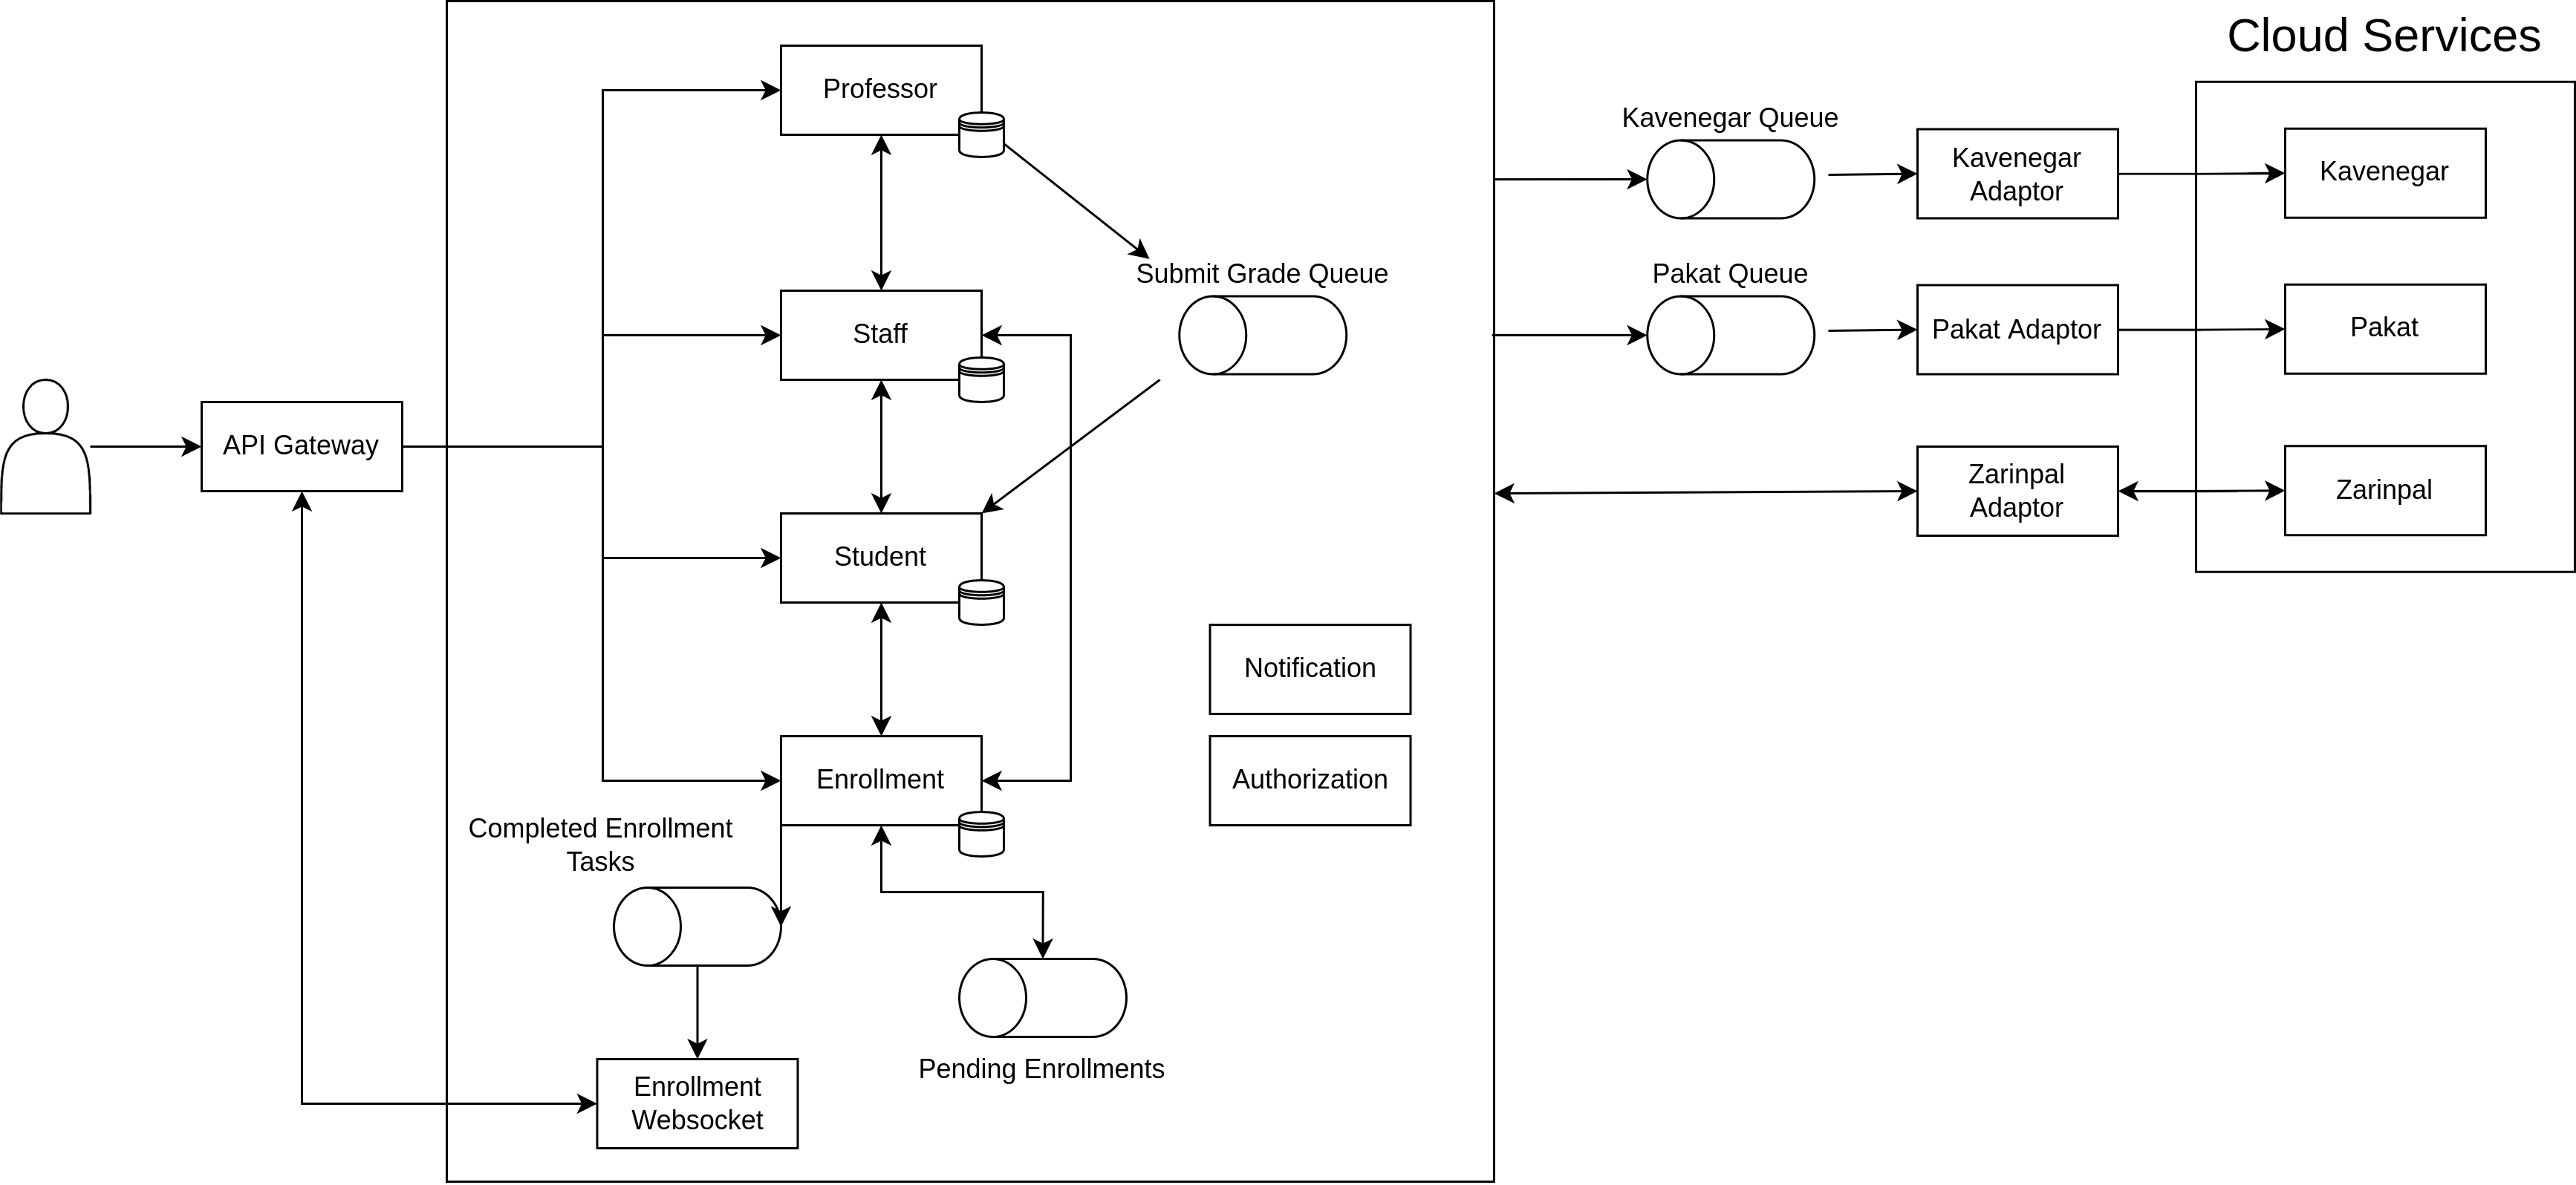
\includegraphics[width=\textwidth,height=\textheight,keepaspectratio]{diagrams/Architecture.png}
    \caption{معماری پیشنهادی سرویس‌ها}
    \label{architecture}
\end{figure}